\documentclass[12pt,twocolumn]{article} %TWO COLUMNS
\usepackage{graphicx}
\usepackage{wrapfig}
\usepackage[hidelinks]{hyperref}
\usepackage{booktabs}
\usepackage{titling} 
\usepackage{abstract}
\usepackage{titlesec}
\usepackage{enumerate}
\bibliographystyle{vancouver}
\usepackage[hmarginratio=1:1,top=15mm,left=15mm,columnsep=15pt]{geometry}% MARGINS
\usepackage[small,labelfont=bf,up,textfont=it,up]{caption} %CAPTIONS FORMAT
%SECTIONS AND SUBSECTIONS
\renewcommand\thesection{\Roman{section}} 
\renewcommand\thesubsection{\roman{subsection}} 
\titleformat{\section}[block]{\large\scshape\centering}{\thesection.}{1em}{} 
\titleformat{\subsection}[block]{\large}{\thesubsection.}{1em}{} 
\titlespacing*{\section}
{0pt}{\baselineskip}{\baselineskip}
% TITLE AND ABSTRACT
\renewcommand{\abstractnamefont}{\normalfont\bfseries}
\renewcommand{\abstracttextfont}{\normalfont\small\itshape}
\pretitle{\begin{center}\Huge\bfseries} 
	\posttitle{\end{center}} 
\title{Problems that arise when peforming a small-scale soil microbiome analysis and how to prevent them} 
\author{\normalsize University College London \\}
\date{\today}
\renewcommand{\maketitlehookd}{
	\begin{abstract}
		\noindent
	 	
	\end{abstract}
}
%INDENTS
\setlength{\parindent}{5mm}
\setlength{\parskip}{0mm}
\setlength{\intextsep}{3mm}
\setlength{\textfloatsep}{5mm}
% DOCUMENT
\begin{document}
	
\maketitle
% IMPROVE THE INTRODUCTION
%
%
\section{Abstract}
Microbiome analysis is an area of research that is currently experiencing a major growth, with over 10000 articles published on the topic in the last 5 years. A severe decrease in price of both the DNA sequencing and computational power in the recent years, led to this data-driven area of research becoming more accessible. In order to determine whether it is possible to generate valid results from a small-scale analysis, 30 samples of soil were collected in Central London and High-Performance Computing clusters were used together with specialised software to assess the uniformity of the samples and discover correlations between the chemical and biological content. This paper will be focused on three main aspects - assessing the validity of the data for further use by other researchers, investigating the relationships that exist between the samples and analysis of the issues that hamper the research on a dataset of low diversity and size.
\section{Introduction}
One of the main areas of development in the field of microbiome analysis in recent years was the creation of big databases with a variety of samples from a range of biomes. The most successful project in this area is the EMP - Earth Microbiome Project\cite{Gilbert2014}. It was started in 2010 and focuses on developing a global catalogue of Earth's microbial diversity, which can be used not only to perform studies on large datasets in order to find correlations within them, but also as a point of reference for specialists in other areas looking for insight into the microbial ecology of different locations and environments. The samples that were collected during our research could potentially be included in the EMP however, the assessment of validity of the genetic sequences extracted should be performed.
\par
The research described in this paper focuses on performing such task, as well as investigating whether a small-scale microbiome analysis, in general, can provide valid scientific results. However, the low number of samples (30) that were collected during this experiment, the low diversity of conditions they were collected in, coupled with inadequate quality of some kits used for analysis created an array of problems. 
\par
%
% METHODS
%
\section{Methods}
The analysis was performed on 30 samples of soil collected in Central London in October 2017.  Metadata, such as moisture, temperature, footfall was collected on the spot, while other aspects such as pH and concentrations of various ions was measured in the laboratory using the \textit{HI3895 Soil testing kit}. Then 4 different kits were used in a workflow designed to extract the sequences of 16S DNA from the prokaryotes in the soil, following the instructions provided by manufacturer of each kit.
\par
First, DNA was extracted using the \textit{DNeasy PowerSoil Kit} and PCR primers were designed that contained Golay barcodes, allowing multiple samples to be sequenced simultaneously. \textit{BioMic PCR kit} was used with the primers to perform the PCR. The solution acquired as the result of PCR was purified using \textit{QIAquick PCR Purification Kit} and then the concentration of dsDNA was measured using \textit{SpectraMax Quant AccuClear Nano dsDNA Assay Kit}. Using the information on DNA concentration all of the samples were subsequently diluted to equal concentrations and sequencing was performed on \textit{Illumina's MiSeq} sequencer. Quality control was performed throughout this stage of the experiment. This workflow returned the DNA sequences that were used for downstream \textit{in silico} analysis.
\par
\textit{In silico} stages of the research were performed using the QIIME\footnote{Version 1.9.1} package\cite{Caporaso2010,Kuczynski2012}, which allows users to perform high-throughput sequence analysis. Parts of analysis that required severe computational power were performed on the Cirrus High-Performance Computing system. QIIME package has basic a pipeline which was used to transform the raw data into the form that can be used for statistical analysis, which is described below.
\par
First step is validation of data, including the mapping and fasta files. After that, sequences are grouped into 30 sets which corresponds to 30 samples. This stage is commonly called demultiplexing, and involves emoval of the barcodes that were introduced in the PCR stage. After the demultiplexed fasta file is produced, OTU (Operational Taxonomic Unit) are picked. OTU picking groups closely related sequences (97\% similarity in our case, which corresponds to species-level sequence identity) into one operational unit, which was used for further analysis.
\par 
OTU picking requires a referencing database, for which SILVA\footnote{Release 132, April 10, 2018}\cite{Quast2012} database was used, which is more up-to-date than Greengenes\cite{McDonald2012} database provided with QIIME. OTU picking and demultiplexing are generally the most expensive stages, in terms of computational power. For this reason they were performed on the Cirrus HPC and most of the downstream analysis was performed on a local machine. 
\par
QIIME package provides a variety of scripts designed to analyse the genetic sequences data. However, it should be noted that while providing a users with variety of methods to perform the analysis, the figures created by the scripts provided are subpar. This lead to creation of a collection of scripts that were used to perform some of the analysis and construct the figures, which can be found on the GitHub repository dedicated to this analysis\cite{Anonymous2018}. The repository also features additional data on the samples that is out of scope of this paper, and was created using various python packages, such as numpy, scipy, pandas, seaborn and matplotlib, which greatly aid in data visualisation and statistical calculations.
\par
A method that is useful to determine whether the samples we collected are representative of the source, is provided in the sourcetracker package\cite{Knights2011}, which allows users to track proportion of each \textit{source} in each \textit{sink}, \textit{source} and \textit{sink} being different samples of soil from Release 1 of the EMP and our samples respectively. Sourcetracker package is available with QIIME, however Sourcetracker2 has been developed recently, which was used due to being more accurate and functional. 
The sourcetracker workflow produces a matrix the displays how much of each source is present in each of our samples was produced.
\par
In an attempt to find a correlation between metadata and the diversity of our samples, scripts included in the QIIME package were used and metadata was transformed into numeric form, with results from \textit{HI3895 Soil testing kit} treated as values on exponential scale. Analysis was performed using ANOSIM\cite{CLARKE1993}, PERMANOVA\cite{Tang2016} and a collection of other statistical methods, which calculate the correlation between the distance matrix and pH, potassium, nitrogen and phosphorus content.
\par
To assess the taxonomic composition of our samples, taxonomic assignment using the SILVA\cite{Quast2012} database was performed. The classical microbiotic analysis was performed as well, that tests the diversity of the samples.
%
% RESULTS
%
\section{Results} 
During the OTU picking stage, over 4.5 million sequences were recovered from raw data, with 16448 of them being unique. However, it should be noted, that due to use of closed-reference OTU picking, almost 800 thousand sequences (17\%) were removed from the downstream analysis because no match was found in the databases. The data is consistent with results obtained in the research performed by Thompson et al.\cite{Thompson2017} on the data from the EMP database, in which they reported that amongst soil samples 20\% of sequences were not identified with SILVA closed-reference OTU picking.
\begin{figure}[ht!] %alpha diversity
	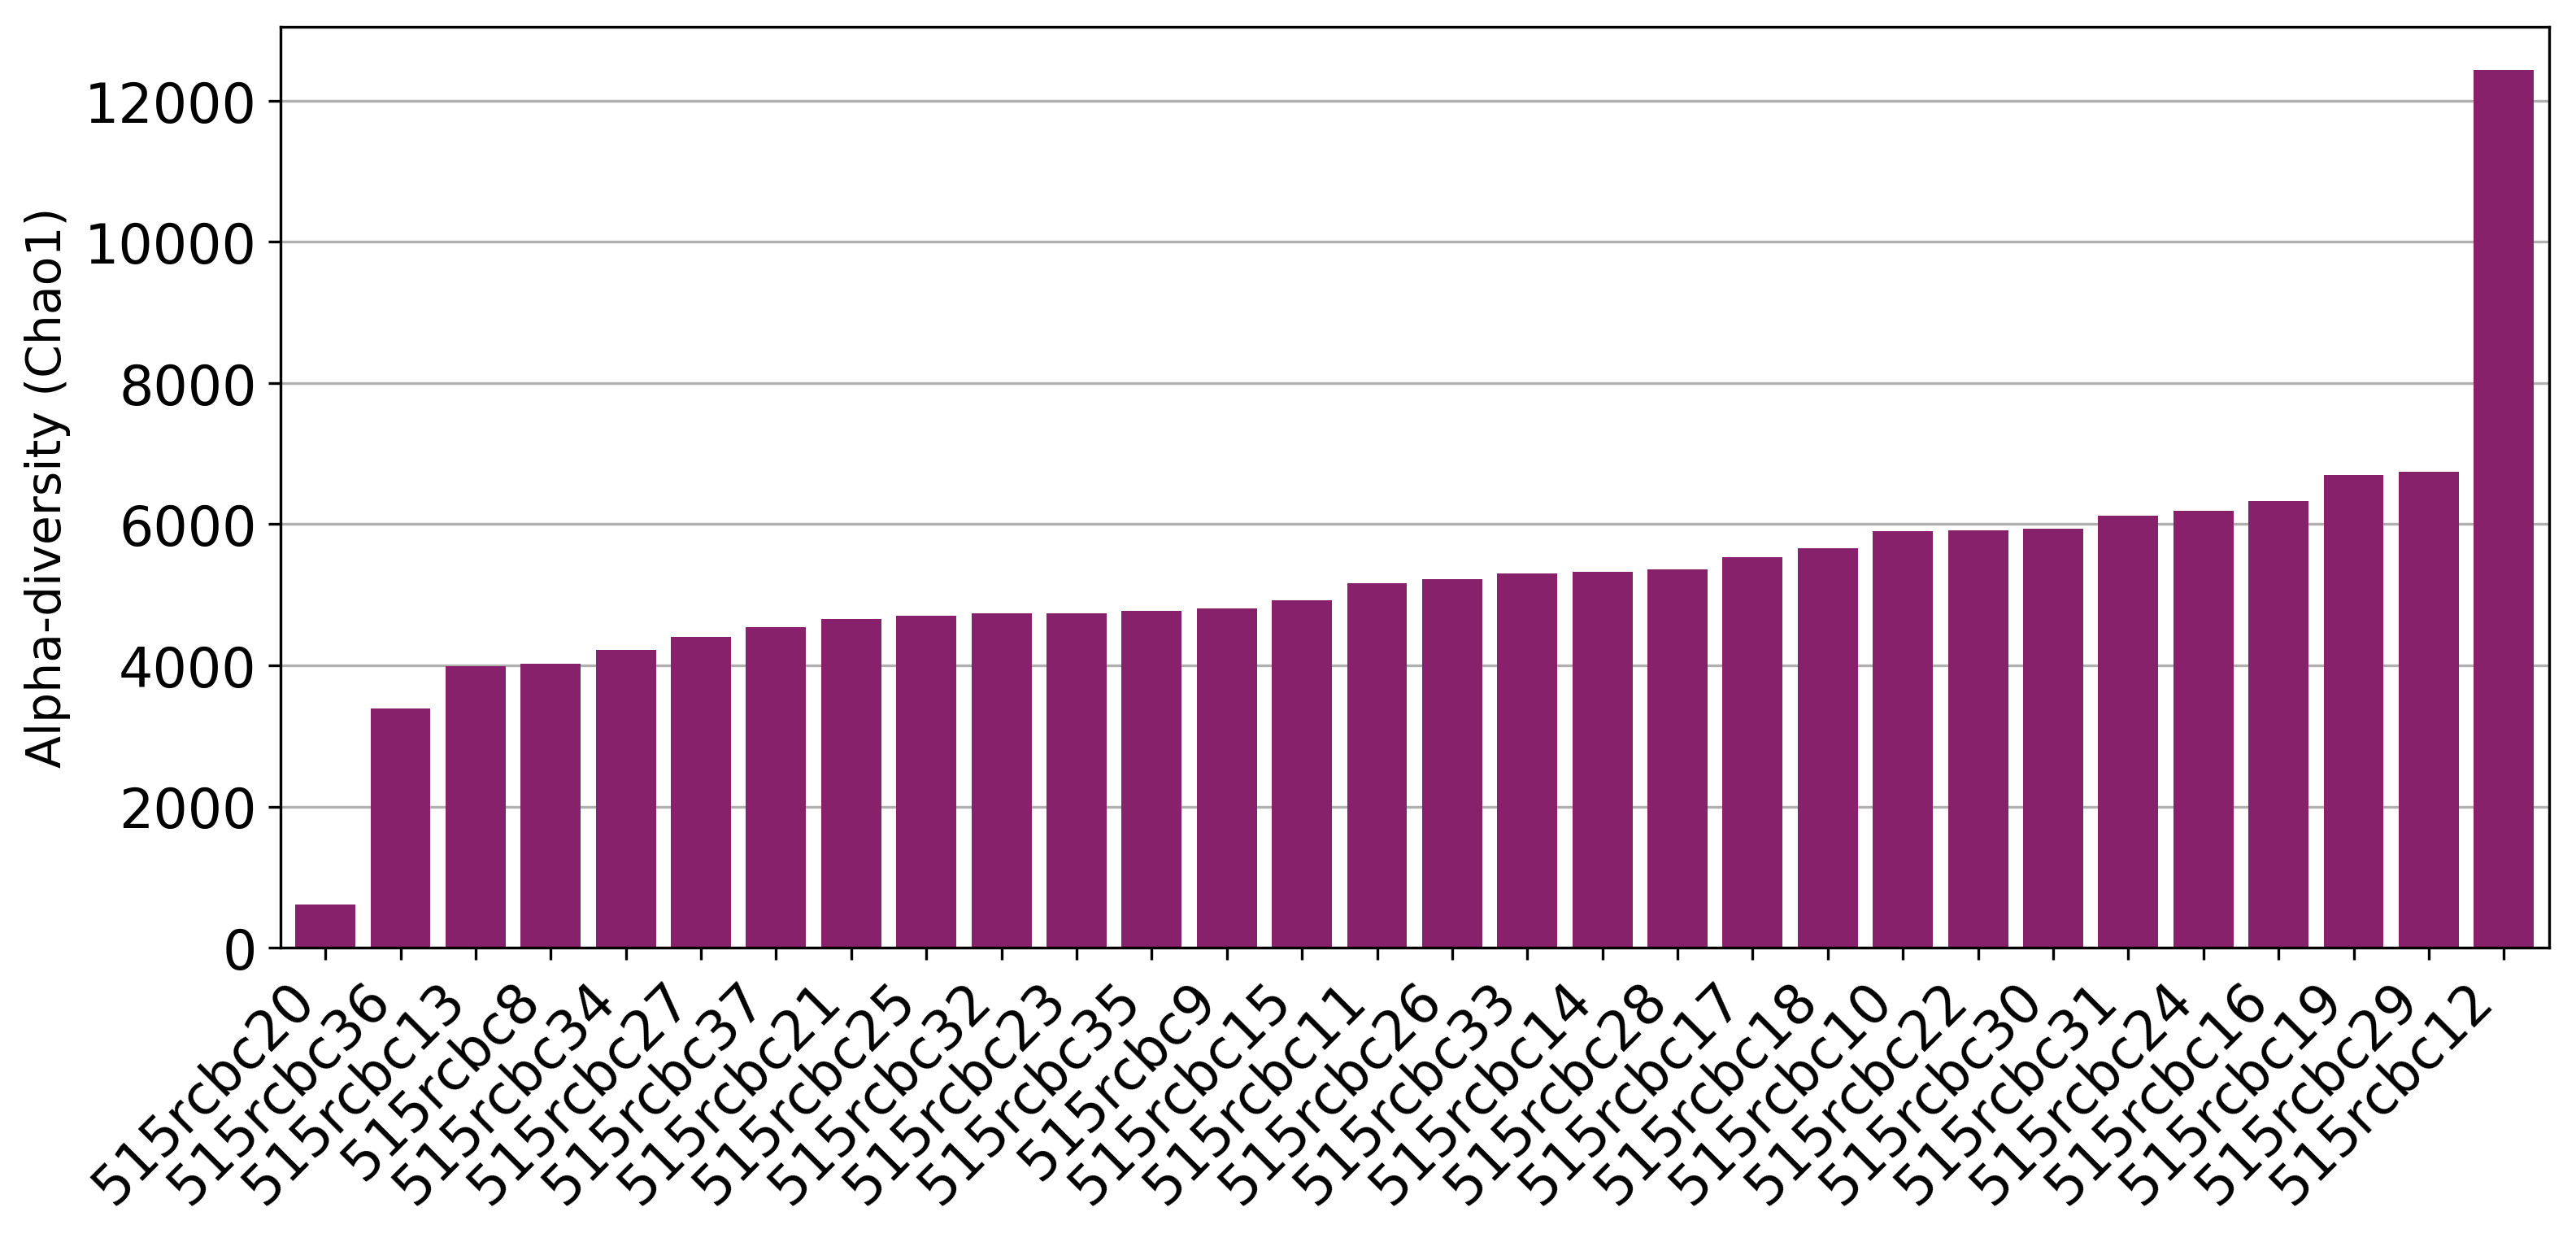
\includegraphics[width=\linewidth]{chao1_alpha.png}
	\caption{Alpha diversity (Chao1) for each of 30 samples. Samples 515rcbc20 and 515rcbc12 exhibit highly distant results, can be explained by their different geographical origin.}
	\label{fig:alpha_diversity}
\end{figure}
\par
Using the OTU table that was produced as a result of the OTU picking, alpha diversity was measured, which assesses the number of unique OTU for each sample. While different methods and metrics can be used, Chao1 was chosen for this test, which estimates species richness based on a matrix of abundance data. The distribution of alpha diversities between the samples is presented below in Figure \ref{fig:alpha_diversity}.
\begin{figure}[ht!] %beta diversity
	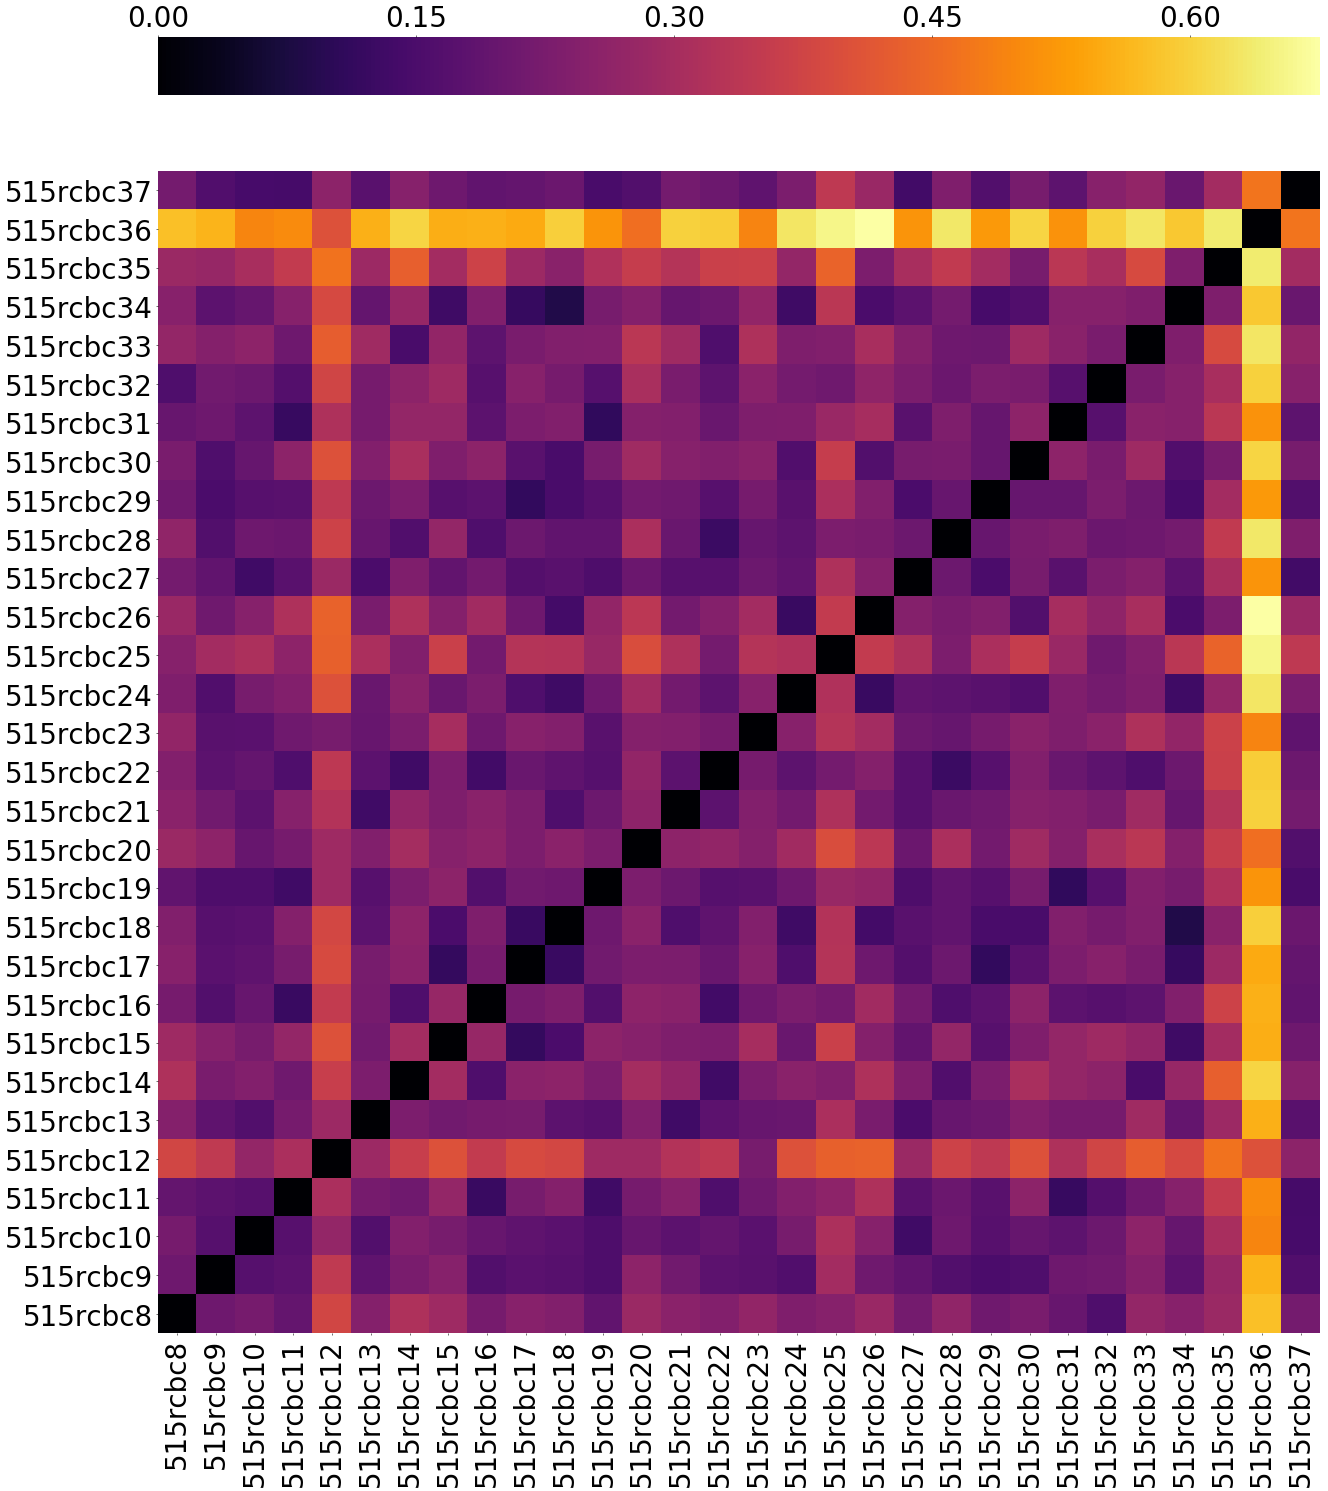
\includegraphics[width=\linewidth]{unweighted_beta.png}
	\caption{Beta diversity (unweighted unifrac) matrix, presented as a heat map. Obvious outliers can be noted again, with samples 515rcbc12 and 515rcbc36 having the largest divergence from other samples.}
	\label{fig:beta_diversity}
\end{figure}
\par
In order to further investigate the uniformity and clustering of the samples, beta-diversity analysis was performed. The heat map presented in Figure \ref{fig:beta_diversity} is a graphical representation of beta-diversity between the samples, with higher values representing higher divergence.
\par
Sample \textit{515rcbc36} can be identified as the most divergent from the rest, with \textit{515rcbc12} being a close contender. While \textit{515rcbc12} has outlying values for the alpha diversity with almost 2-fold difference in alpha diversity compared to all other samples, \textit{515rcbc36} does not exhibit any severe difference in other results when compared to the rest. Moreover, \textit{515rcbc12} was collected in a different geographical location and different conditions, which can explain its high beta-diversity scores however, \textit{515rcbc36} was collected in conditions that are identical to other samples. This leads to the assumption that that this sample was contaminated. This assumption is backed up by the taxonomical assignment of OTUs, which shows that sample \textit{515rcbc36} has different proportions of various taxa compared to other samples.
\begin{table}[ht!] %statistical table
	\begin{center}
		\label{tab:table_correlation}
		\begin{tabular}{c|c|c}
			\textbf{Category} & \textbf{R-value} & \textbf{p-value}\\
			\hline
			pH & -0.109 & 0.869\\
			Potassium & 0.224 & 0.023\\
			Nitrogen & 0.120 & 0.120 \\
			Phosphorus & 0.201 & 0.058\\
		\end{tabular}
		\caption{Correlation between metadata and beta-diversity, calculated using ANOSIM\cite{CLARKE1993} method.}
	\end{center}
\end{table}
\par
Despite the two aforementioned samples being the obvious outliers, sample \textit{515rcbc20}, which was collected in different conditions and displayed an atypical alpha diversity does not differ severely from the other samples on this heat map. This happens due to the nature of unweighted unifrac beta diversity metric - it takes into account the total number of OTUs in the sample, thus nullifying the difference in the total number of samples.
\par
In order to determine whether the data obtained in a small-scale microbiome analysis is enough to find correlations between the metadata and diversity, several statistical analyses were performed. First, statistical method of ecology analysis ANOSIM\cite{CLARKE1993} was used together with the collected metadata and distance matrices to find any correlations, results are presented in Table 1.
\par
Since the R-value is close to 0 for all four metrics, it can be safely assumed that there is no statistically significant correlation between metadata and the diversity in our samples. Other methods of statistical analysis, such as PERMANOVA\cite{Tang2016} confirmed this assumption, attempts to find non-linear correlations were not successful as well.

\par
The assessment of taxonomic composition of the samples was performed as well, with the taxonomic referencing database included in the SILVA database used to assign taxonomy to most of the OTUs. Figure \ref{fig:top_taxa} highlights the top 10 most abundant phyla across all of the samples. These 10 phyla represent 96\% of the sequences. More detailed plots on the topic of taxonomy are also available on GitHub\cite{Anonymous2018}.
\begin{figure}[ht!] %top phyla
	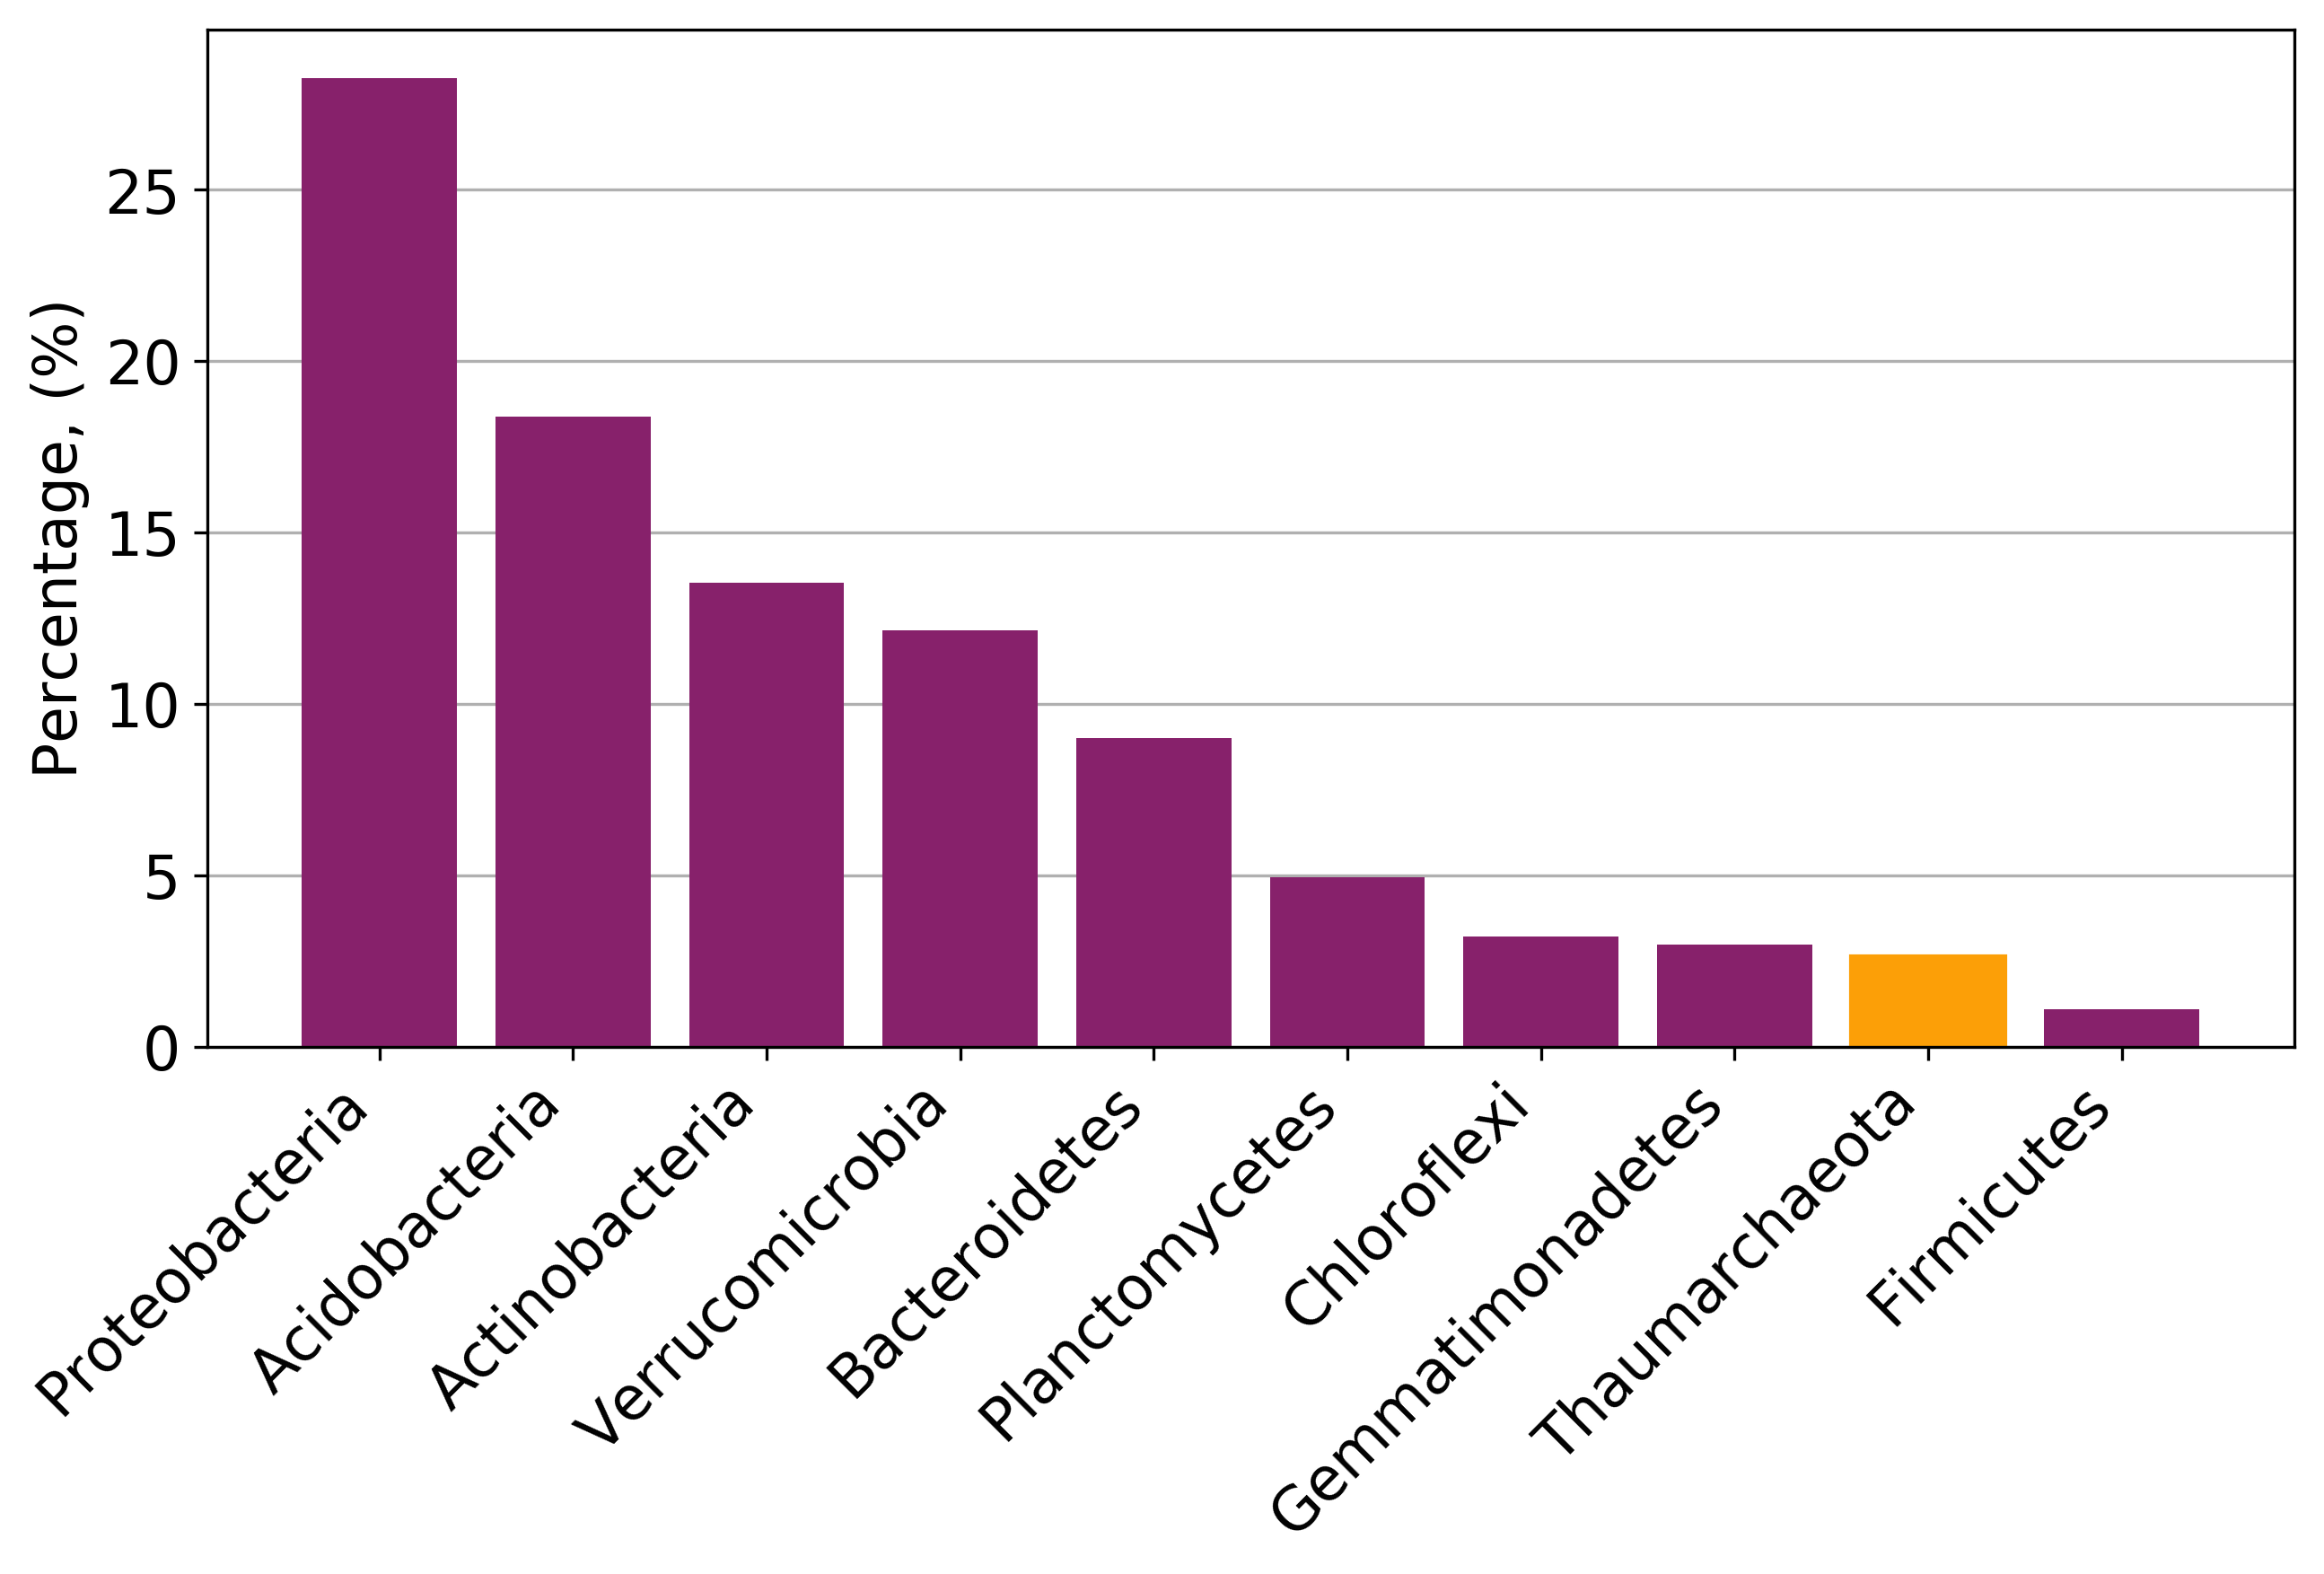
\includegraphics[width=\linewidth]{top_10.png}
	\caption{Proportion of most popular phyla in samples. The orange bar represents the only phylum from the Archea domain. These 10 phyla represent 96\% of species in our samples.}
	\label{fig:top_taxa}
\end{figure}
\par
The only phylum from the \textit{Archea} domain is \textit{Thaumarchaeota} and the rest of the  sequences have a bacterial origin. This is consistent with a similar research conducted by Zhalnina et al.\cite{Zhalnina2014}, in which they investigated the taxonomy of the Park Grass Experiment. The proportions of the most abundant phyla is similar, which speaks in favour of the validity of our samples.
\par
The sourcetracker package was employed to assess the relatedness of our samples to samples of soil from different biomes around the world collected by the researchers working on the EMP projects . Sourcetracker exploits a mathematical approach which assesses the proportion of each \textit{source} in each \textit{sink}. The results are a matrix , which is presented in Figure \ref{fig:sourcetracker_heatmap} as a heat map . 
\begin{figure}[ht!] %sourcetracker
	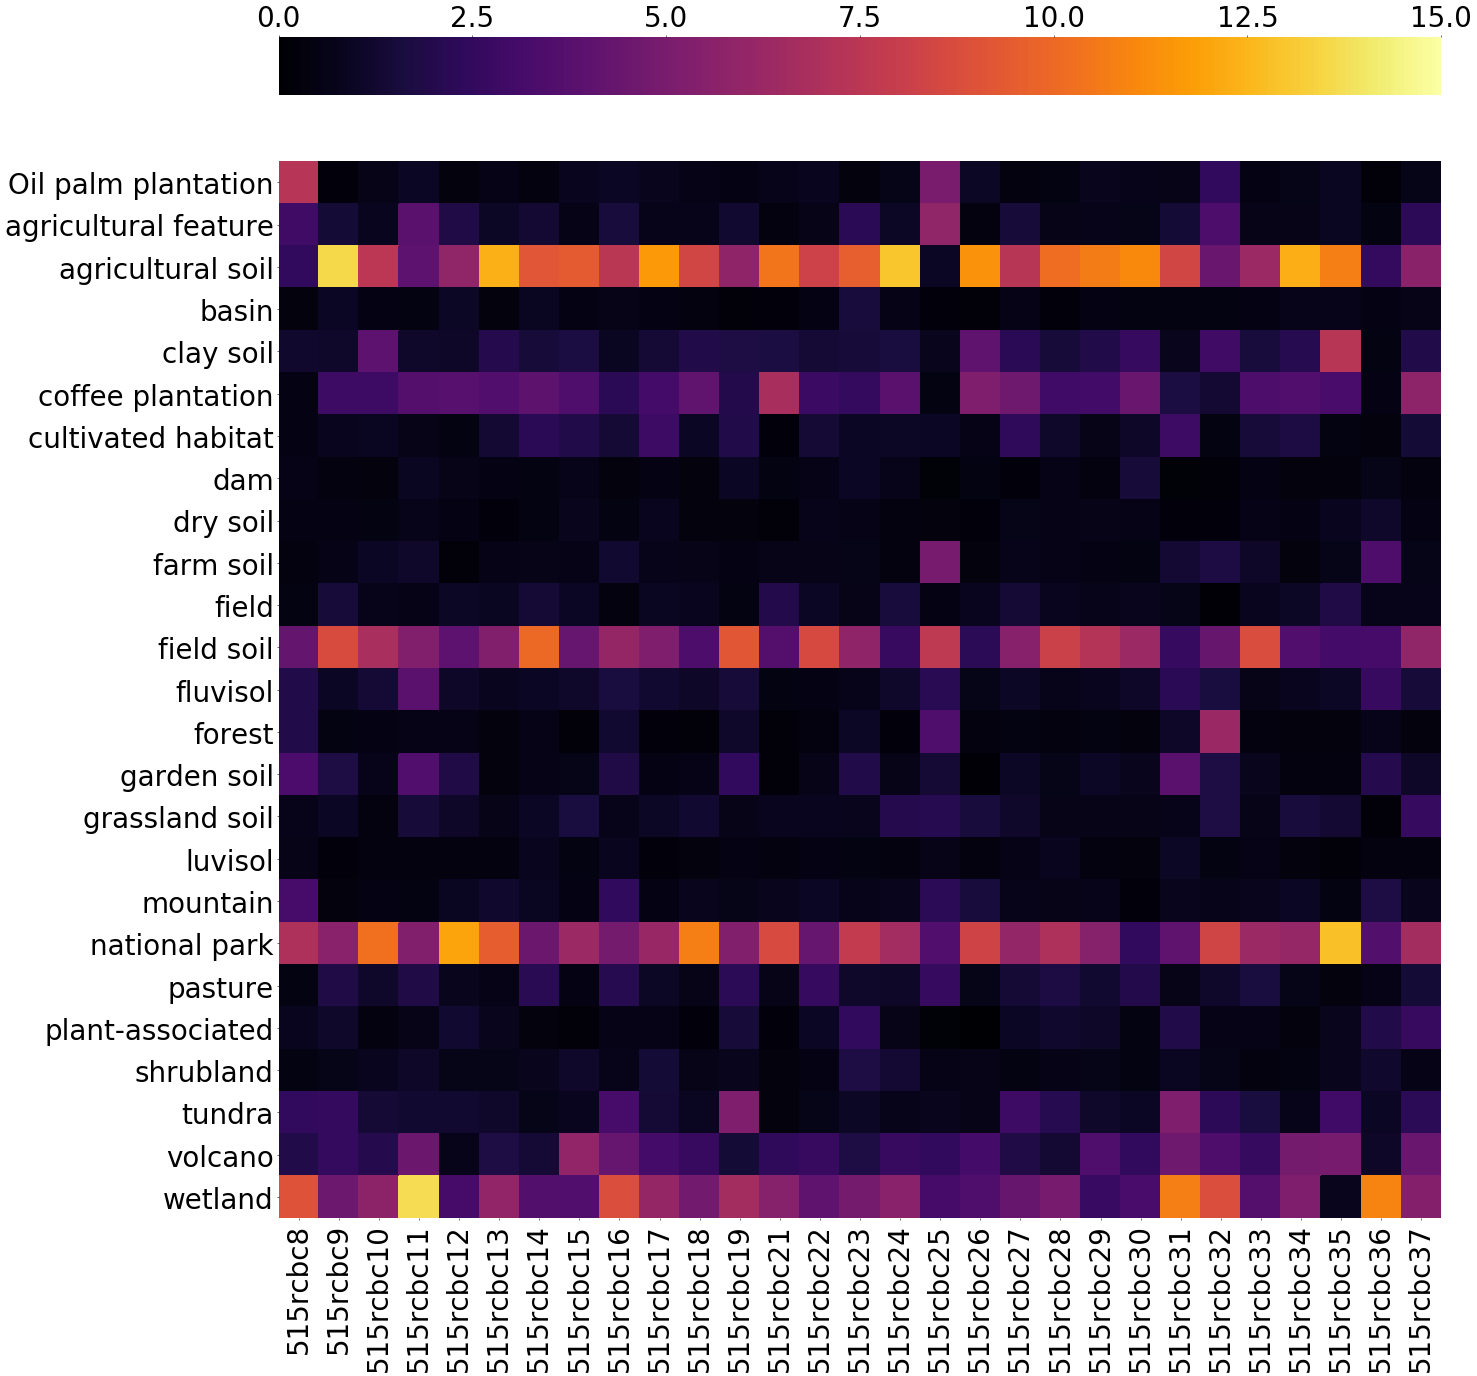
\includegraphics[width=\linewidth]{heatmap_perc.png}
	\caption{Heat map showing the percentage of each source in each sink, filtered to represent the top 25 sources. The "Unknown" column is not presented as well, it represents a mean of 44\% of sources in each sink. As we can see there are 4 prominent sources in most sinks - agricultural soil, national park soil, wetland soil and field soil, which have a mean percentage of over 5\%.}
	\label{fig:sourcetracker_heatmap}
\end{figure}
\par
The heat map shows that most samples have high relatedness to 4 different biomes - national park soil, field soil, agricultural soil and wetland. Sample \textit{515rcbc20} had to be excluded from the analysis due to low number of OTUs observed (653). Our samples were collected in Gordon Square in Central London, a biome that is anthropomorphic, which can explain the high relatedness to agricultural soil and field soil. The unifying feature of such environments is heavy use of fertilizers, which leads to development of a specific ecosystem\cite{Zhalnina2014}. This further reinforces the hypothesis that except for a small number of outliers mentioned above, the samples present genetic data of a high enough quality to be included in the EMP.
\par
Despite the peculiarity of some results of the sourcetracker analysis, in general it confirms the uniformity and good clustering of the the samples. Low number of samples collected prevents us from making any further assumptions about the outliers and peculiar correlations between the EMP soil data and the samples, and further research is required to explain high proportion of wetland source in many samples and other aberrations.
\par

%
% DISCUSSION
%

\section{Discussion}
The results of the first steps in the computational pipeline show that the approach based on OTU picking does not provide the most accurate results. For instance, the SILVA database currently contains 177222 sequences, which means that our study, while being rather small, covered almost 10\% of the database. Thompson et al.\cite{Thompson2017} report that a study they performed using just under 100 samples from different biomes covered  47\% of the SILVA database. Low coverage of even the most up-to-date databases such as SILVA combined with the diminishing property of the OTU picking process creates the need for more accurate methods of sequence assessment, such as Deblur\cite{Amir}. 
\par
As we can see from the results of alpha and beta diversity analysis, our samples form a uniform collection, with samples \textit{515rcbc12}, \textit{515rcbc20} and \textit{515rcbc36} forming an array of abberations. And while the first two were expected outliers due to the altered condition they were collected in, sample \textit{515rcbc36} is an unpredicted outlier, since it had an identical metadata to other samples. However, further analysis is required to prove test the hypothesis that this sample was contaminated.
\par
The uniformity and tight clustering of the samples, while validating the dataset for comparison with other datasets at the same time hinders any attempts to discover correlations between the genetic data and metadata. In order to find any correlation a purposeful diversification of samples is required, such as variance of location, season or other conditions. Since 27 of the samples were collected in the same location at the same time, there is very low variance in the samples and the few outliers can only provide anecdotal evidence. If a similar experiment is to be performed by other researchers, diversification of samples should be considered a paramount step.
\par
In addition to diversification of samples, high-grade methods of metadata collection are required. While the kits that were provided by University College of London give a general idea of concentrations of various ions in the soil, they do not match the level of this research.
\par
In conclusion, it must be noted that the samples provide a good addition to the existing microbiome databases such as EMP, since it was confirmed by multiple \textit{in silico} tests that the protocol of extracting the DNA from samples was executed without major complications. However, stand-alone scientific value of the dataset is minuscule, due to absence of correlation between the chemical composition of the samples and the DNA sequences extracted. In order to obtain data that can provide researchers with statistically significant results, the diversity of samples, methods of metadata collection must be improved and use of reference-free sequence analysis techniques is preferential.
 


\bibliography{/home/ilya/Documents/Citations/3301.bib}
\end{document}